\chapter{RESULTS AND DISCUSSIONS}
\label{chp:results-and-discussions}

In this chapter, methodology presented in this thesis study is applied on datasets and results are presented. Firstly, evaluation metrics are defined for each stage of methodology to evaluate performance of the approach. Following this, methodology is applied on two datasets and results are explained with discussions.

\section{Evaluation Metrics}
\label{sec:evaluation-metrics}
Approach in this study is an aggregation of various methods and they are significantly different from each other in their mathematical background. Therefore, instead of a global evaluation metric for the complete methodology, each stage will be evaluated within its evaluation metrics. Since these stages are executed sequentially, it is important for each stage to perform enough well to yield a successful outcome. In this section, evaluation metrics for each stage will be presented and they will be used to determine the success of methodology on experiments.

\subsection{Process Model Mining}
\label{subsec:process-model-mining-eval}
Process model mining stage takes input as event logs of organizations and creates process models using process mining algorithms, namely \textit{Inductive Miner} \cite{leemans2014discoveringinfrequent}. Performance of this stage can be measured by the conformance of the process models to the the event logs. Four competing quality criteria are defined in \cite{van2011process} and they are \textit{fitness}, \textit{simplicity}, \textit{precision} and \textit{generalization}. Fitness is based on the idea of being able to replay event log over process model whereas precision focuses not underfitting the event log. Simplicity idea is based on the fact that the simplest model is the best model, on the other hand generalization supports not overfitting the event logs. These four competing criteria are mathematically defined in \cite{rozinat2008conformance} and grouped into two dimensions for analysis purposes:

\begin{description}
  \item[Fitness] Event log and the process model should \textit{fit} to each other, in other words process model should be able to parse the event log. 
  \item[Appropriateness] Since \textit{fitness} does not provide information about the meaningfulness of process models, this dimension is defined. Two notions comprise this idea; \textit{Structural Appropriateness} considers the simplicity whereas \textit{Behavioral Appropriateness} analyzes balance between overfitting and underfitting.
\end{description}

In this thesis study, process model mining stage will be evaluated by the \textit{Fitness} and \textit{Appropriateness} of the mined process models for each organization. In ProM  It is expected to have higher \textit{fitness}, closer to 1, and a high level of appropriateness to continue to the next stages with the high quality process models. While evaluating, \textit{fitness} will be more dominant since \textit{appropriateness} without \textit{fitness} means less.
%	conformance plugin'i çağır, filtre ekranında var, 
%	structural olanı elle hesapla -> http://wwwis.win.tue.nl/~wvdaalst/publications/p436.pdf pg21
\subsection{Performance Indicator Analysis}
\label{subsec:performance-indicator-analysis-eval}
Performance indicator analysis stage consists of two parts as replaying event logs over process models and clustering organizations based on the performance indicators. In the replay phase, main operation is to \textit{align} \cite{van2012replaying} event logs and process models. This alignment is the based on the idea of finding the optimal alignment where total cost of \textit{move on process model} and \textit{move on event log} are minimized. Since there is no baseline information for alignment costs of organizational logs, total cost information will be used together with the process model mining evaluation metrics. In other words, for the event logs and process models with known conformance metrics, total cost of alignments will create a secondary check if there are any problems related to replaying events over process models. It is expected to have less total cost of alignment for the organizations with higher conformance since it is easy to align event logs and processes with high superior fitness values.
% Şu pluginle bak: Check compliance using conformance checking ->
For the second stage of performance indicator analysis, there is a need to evaluate performance of clustering organizations. In this stage, organizations are clustered  based on their performance indicator values that are calculated over replaying. Since there is no labeled data in the context of this thesis study, any cross-validation techniques could not be applied and thus internal evaluation metrics are exploited. As mentioned in the Section~\ref{subsec:performance-indicator-clustering}, within SSE values between clusters are plotted to the end user to select an appropriate number of clusters. It is expected that within SSE values decreases as number of clusters increases; however, number of clusters should be selected without causing overfitting.
% wekadan gelen within sse 

\subsection{Mismatch Pattern Analysis}
\label{subsec:mismatch-pattern-analysis-eval}
Mismatch pattern analysis stage aims to find differences between the process models of different organizations. In this thesis study mismatch patterns defined in \cite{dijkman2007mismatch} are mathematically defined and analyzers are developed to locate these patterns. At the time of this study, it is known to be first to use mismatch patterns in a generic method, therefore evaluation is based on comparing with well-defined prior similarity metrics.

Structural similarity between process models is presented in \cite{dijkman2011similarity} by the \textit{graph-edit distance} notion. In graph theory, \textit{graph-edit distance} is the minimum number of \textit{graph-edit operations} necessary to get one from graph to another. In the process mining field, \textit{graph-edit operations} are simply node addition, deletion or substitution. In the study \cite{dijkman2011similarity}, both \textit{graph-edit distance} and \textit{graph-edit similarity} definitions are provided with their mathematical background. In this study, mismatch pattern analysis stage is evaluated by comparing the number of mismatch patterns and the \textit{graph-edit similarity} of process models. Without any performance indicator clustering, it is expected to have larger number of mismatch patterns when the similarity between process models is low. This will ensure the performance and suitability using mismatch pattern analysis instead in the methodology.
 % BartHompes paketi ile ikili ikili çalıştır- run
\subsection{Recommendation Generation}
\label{subsec:recommendation-generation-eval}
In the recommendation generation stage, set of mismatch patterns are presented to the end user based on the selected organization and performance difference threshold. This stage aims to list whole mismatch patterns that can cause the other organizations perform better than a difference threshold. Idea of using performance threshold should be evaluated in this stage with its responsiveness. In other words, it is expected that this stage will help the end user to focus on the most important performance improvements for the organization analyzed. Therefore, different threshold values will be tried to check how many mismatch patterns are generated for organizations and how they could be used for focused analysis. In addition, quality and applicability of the recommendations should be analyzed and this requires a high level of knowledge starting from the collecting event logs in the organizations. This knowledge should include know-how about process changes, domain knowledge about the field of organizations' activity and structural attributions of the organizations.

\section{Dataset Selection}
\label{sec:dataset-selection}
Cross-organizational mining aims to find cross-correlation of workflows and activities in different organizations and this yields the necessity of organizations that do the same main activity with a comparable process flows. In business life, this includes aligning the tasks from different organizations with different business needs, priorities and organizational structures and culture. Considering these characteristics, there are few dataset available in the literature that are well-structured, documented and valuable. In this thesis study, one synthetic and one real-life event log datasets  are presented and used in the following sections to evaluate the performance of the proposed methodology.

\begin{description}
  \item[Loan Application Process \cite{loan-app-data}] This synthetically created dataset consists of event log variants of a simple loan application in a financial institute. In summary, a customer fills a form and starts a request over website and it starts the different approaches of variants in different organizations that ends with notifying the customer about the acceptance of application. This dataset includes artificial event logs of 4 variants where each variant includes different sets of approaches such as parallelism, choices and sequential tasks. These event logs are used to test different approaches of discovering a configurable process model from a collection of event logs in study \cite{buijs2014flexible}.
  \item[Environmental Permit Application Process \cite{coselog-data}] This dataset originates from the "Configurable Services for Local Governments (CoSeLoG)" project \cite{van2011business} which investigates the similarities and dissimilarities between several processes of different municipalities in the Netherlands.  Dataset contains the records of the execution of the receiving phase of the building permit application process in 5 municipalities, which are comparable since activity labels in the different event logs refer to the same activities performed in five municipalities. This data set is also mentioned in the literature as \textit{"Processing applications for building and/or environmental permits (Wet Algemene Bepalingen omgevingsrecht (WABO) in Dutch)"}.

  When the organizations that have similar processes are considered, municipalities are one of the prominent candidates. In Netherlands there are more than 400 municipalities and they offer between 400 and 500 different products and services with their own processes. Unlike corporations, municipalities have the advantage that they can seek for collaboration since they are not direct competitions \cite{buijs2012towards} and this advantage makes them valuable for cross-organizational analysis. CoSeLoG research project aims to develop a business process management system within a shared Software-as-a-Service environment using the commonalities between the processes of municipalities \cite{buijs2014flexible}. In the scope of CoSeLoG research, five different processes of municipalities are analyzed and at the time of this thesis study only \textit{Environmental Permit Application Process} dataset is publicly shared.
\end{description}

\section{Loan Application Process}
\label{sec:loan-app-process}

\subsection{General Information}
\label{sec:loan-app-information}

In this section, methodology proposed in this thesis study will be applied on the \textit{Loan Application Process} dataset \cite{loan-app-data} and evaluation results will be presented. Statistical information about this dataset is presented in Table~\ref{table:loan-app-process-summary} to provide an insight about this dataset.
%\caption{Statistical summary of Loan Application Process Dataset}
%\label{table:loan-app-process-summary}
\begin{table}[]
\centering
\caption{Statistical summary of Loan Application Process dataset}
\label{table:loan-app-process-summary}
\begin{tabular}{@{}lccc@{}}
\toprule
                  & {\bf Cases} & {\bf Events} & {\bf Percentage} \\ \midrule
{\bf Variant \#1} & 100         & 590          & 24 \%            \\ \midrule
{\bf Variant \#2} & 70          & 420          & 17 \%            \\ \midrule
{\bf Variant \#3} & 200         & 800          & 33 \%            \\ \midrule
{\bf Variant \#4} & 105         & 630          & 26 \%            \\ \midrule
{\bf Total}       & {\bf 475}   & {\bf 2440}   & {\bf }           \\ \bottomrule
\end{tabular}
\end{table}

As shown in Table~\ref{table:loan-app-process-summary}, total of 475 cases and 2440 events included in this dataset with a fairly even distribution between variants. In the following section, these variants will be used as organizational logs and the methodology presented in this thesis study will be applied.

\subsection{Methodology Stages}
\label{sec:loan-app-methodology}
In \textit{Process Model Mining} stage, variants of the dataset are used as organizational event logs and they are used to mine process models. Since dataset is synthetically generated, noise threshold in \textit{Inductive Miner} is set to 0 and perfect log fitness is ensured. Appropriateness and fitness evaluation metrics are summarized in Table~\ref{table:loan-app-process-process-model-mining} and it can be seen that each event log is successful in terms of representing reality and being appropriate as a process model. Especially for the variants other than Variant \#1, there is a perfect fitness and appropriateness as it is expected from a  synthetically generated dataset without noise. In addition, process models for each event log is visualized in Figure~\ref{fig:loan-application-process-models}.
%\caption{Process Model Mining Evaluation of Loan Application Process Dataset}
%\label{table:loan-app-process-process-model-mining}
\begin{table}[]
\centering
\caption{Process Model Mining Evaluation of Loan Application Process Dataset}
\label{table:loan-app-process-process-model-mining}
\begin{tabular}{lcccc}
\hline
 & {\bf Fitness} & {\bf \begin{tabular}[c]{@{}c@{}}Structural\\Appropriateness\end{tabular}} & {\bf \begin{tabular}[c]{@{}c@{}}Behavioral\\Appropriateness\end{tabular}} & {\bf \begin{tabular}[c]{@{}c@{}}Average\\Appropriateness\end{tabular}} \\ \hline
{\bf Variant \#1} & 100 \% & 70 \% & 98.5 \% & 84.2 \% \\ \hline
{\bf Variant \#2} & 100 \% & 100 \% & 100 \% & 100 \% \\ \hline
{\bf Variant \#3} & 100 \% & 100 \% & 100 \% & 100 \% \\ \hline
{\bf Variant \#4} & 100 \% & 100 \% & 98.2 \% & 99.1 \% \\ \hline
{\bf Average} & {\bf 100 \%} & {\bf 92.5 \%} & {\bf 99.7 \%} & {\bf 96.06 \%} \\ \hline
\end{tabular}
\end{table}
\begin{figure}
\centering
  \begin{subfigure}{.4\textwidth}
    \centering
    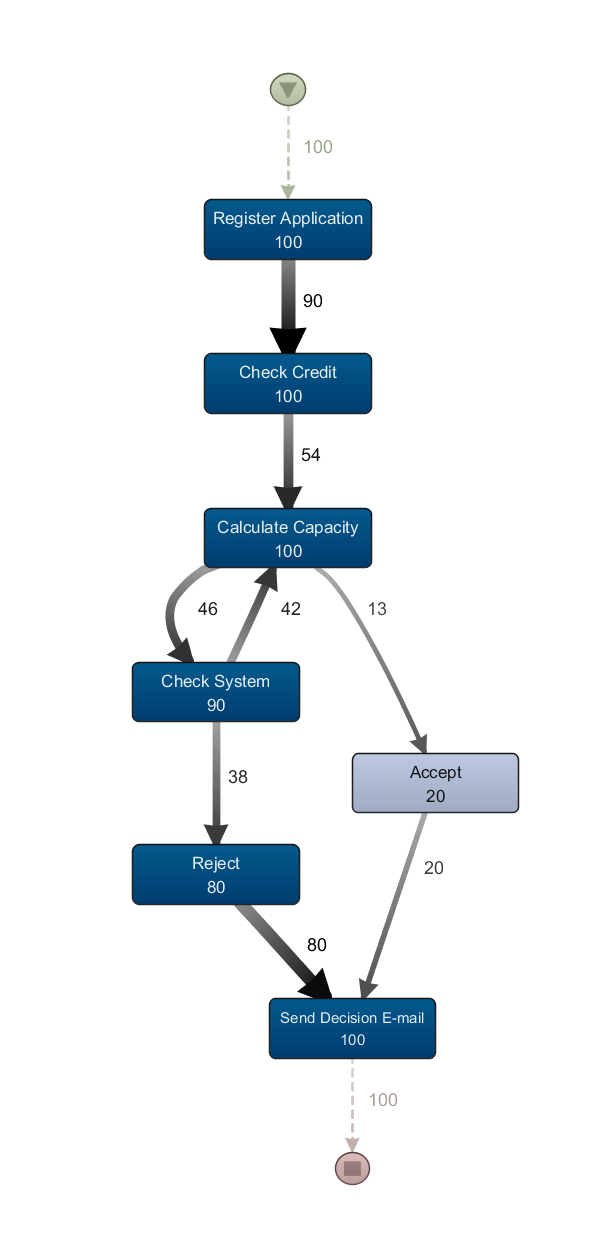
\includegraphics[width=.8\linewidth]{5_results_discussions/loan-application-process/ETM_Configuration1}
    \caption{Variant \#1}
    \label{fig:loan-application-process-models-1}
  \end{subfigure}%
  \begin{subfigure}{.4\textwidth}
    \centering
    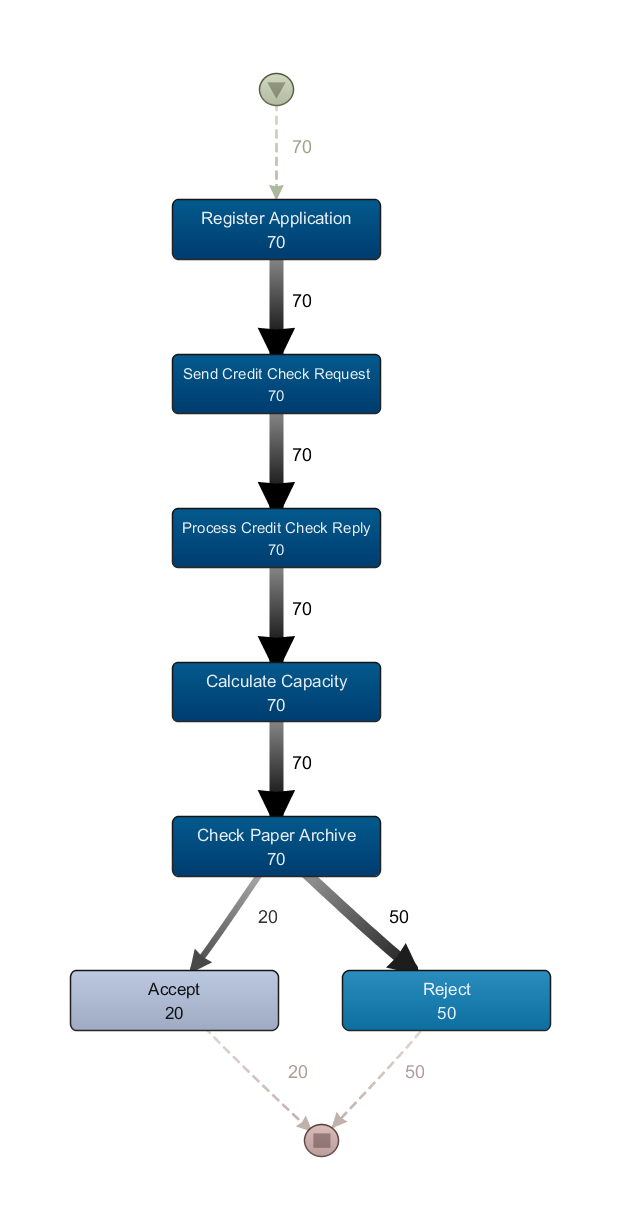
\includegraphics[width=.8\linewidth]{5_results_discussions/loan-application-process/ETM_Configuration2}
    \caption{Variant \#2}
    \label{fig:loan-application-process-models-2}
  \end{subfigure} \\
  \begin{subfigure}{.4\textwidth}
    \centering
    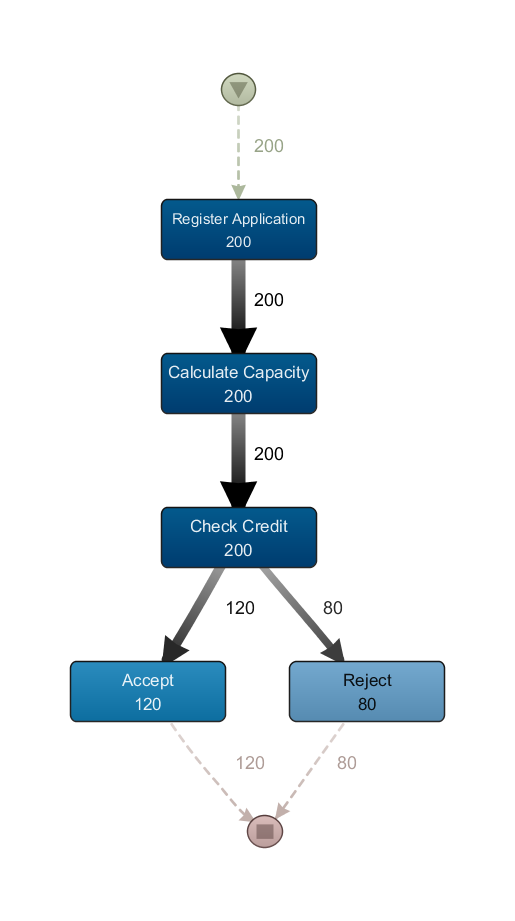
\includegraphics[width=.8\linewidth]{5_results_discussions/loan-application-process/ETM_Configuration3}
    \caption{Variant \#3}
    \label{fig:loan-application-process-models-3}
  \end{subfigure}%
  \begin{subfigure}{.4\textwidth}
    \centering
    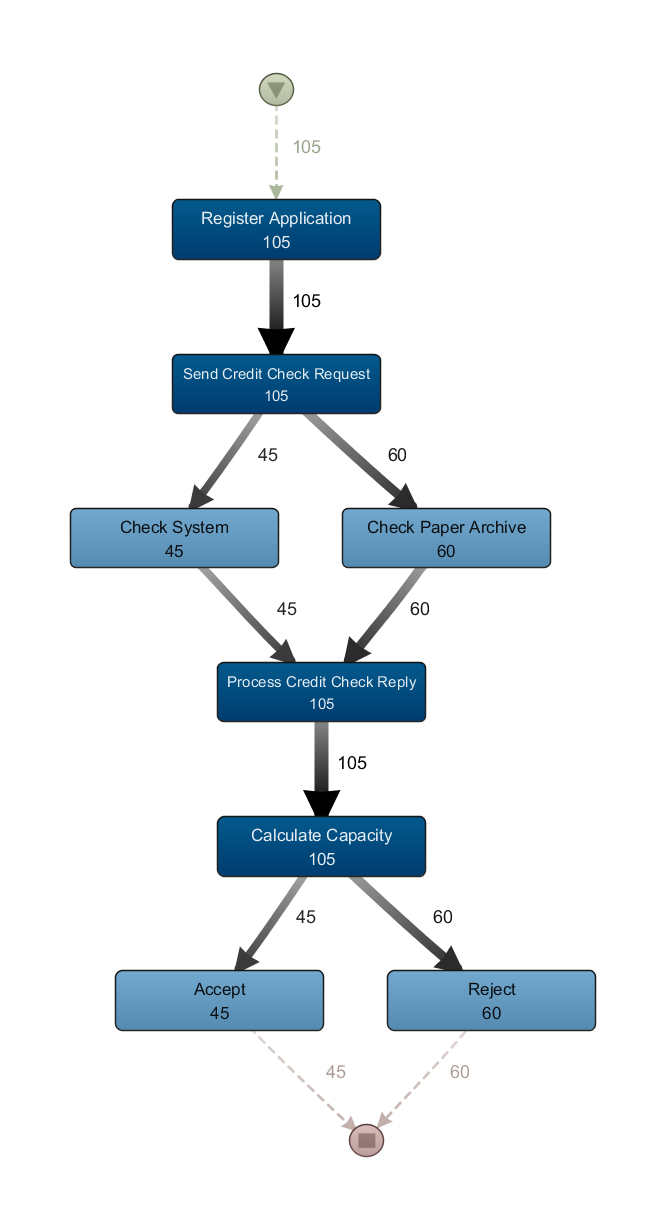
\includegraphics[width=.8\linewidth]{5_results_discussions/loan-application-process/ETM_Configuration4}
    \caption{Variant \#4}
    \label{fig:loan-application-process-models-4}
  \end{subfigure}
\caption{Process models of Loan Application Process dataset}
\label{fig:loan-application-process-models}
\end{figure} 

In \textit{Performance Indicator Analysis} stage, firstly event logs are replayed over process models and performance indicators are calculated. For replaying step, alignment costs should be checked with respect to process model mining evaluation metrics; however, since all fitness values of variants are 100 \% in Table~\ref{table:loan-app-process-process-model-mining}, corresponding alignment costs are 0 for this dataset. This ensures that event logs are successfully replayed over process models and performance indicators are calculated. With these performance indicators, organizations are clustered and internal evaluation of clusters are presented with different number of clusters in Figure~\ref{fig:loan-cluster-sse-plot}. As expected, within-SSE value decreases when number of clusters, \textit{k}, increases. Considering the effects of overfitting after the \textit{elbow} point in the plot, number of clusters is selected to be 2 for this dataset. For two clusters, Variant \#1, \#2, and \#4 are grouped into one cluster where only Variant \#3 is left to other cluster.
\begin{figure}
	\centering
	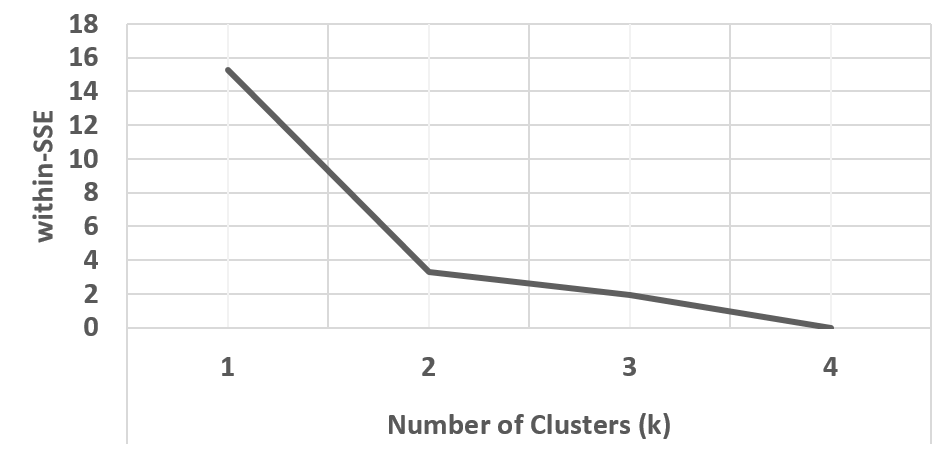
\includegraphics[width=.7\textwidth]{5_results_discussions/loan-application-process/cluster-sse-plot}
	\caption{Number of Clusters vs. within-SSE for Loan Application Process dataset}
  \label{fig:loan-cluster-sse-plot}
\end{figure}

In \textit{Mismatch Pattern Analysis} stage, number of mismatch patterns are analyzed with the \textit{graph-edit similarity} between each two organization. For each two organization, their \textit{graph-edit similarity} values are calculated and then our mismatch pattern analyzers are executed to spot differences. As the similarity between process models decreases our method spots more mismatch patterns for most of the variants and it ensures that the developed mismatch pattern analyzers work as expected for this dataset. Correlation between \textit{graph-edit similarity} and number of mismatch patterns are plotted in Figure~\ref{fig:loan-mismatch-pattern-analysis-results}.
\begin{figure}
	\centering
	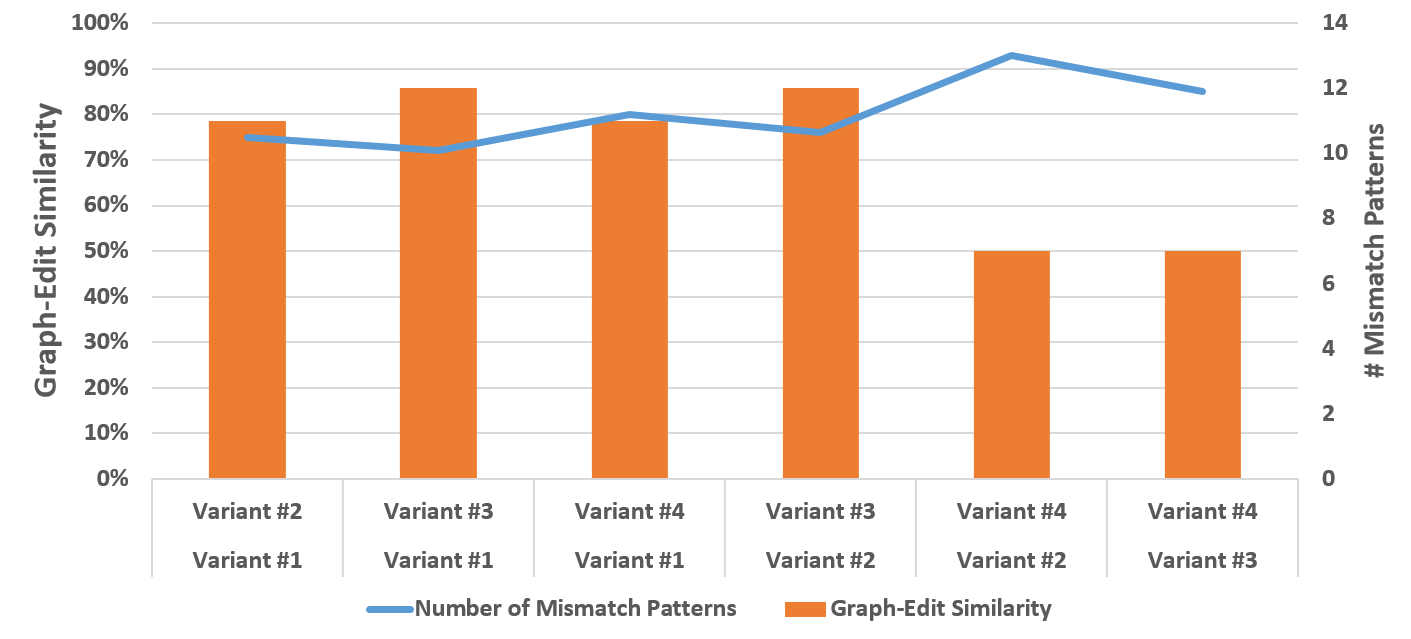
\includegraphics[width=\textwidth]{5_results_discussions/loan-application-process/mismatch-pattern-analysis-results}
	\caption{Mismatch Patterns vs. Graph-Edit Similarity for Loan Application Process variants}
  \label{fig:loan-mismatch-pattern-analysis-results}
\end{figure}

When the mismatch patterns are analyzed according to their types as diagrammed in Figure~\ref{fig:loan-mismatch-pattern-types}, \textit{"Skipped Activity"} and \textit{"Activities at Different Moments"} patterns are spotted mostly and no \textit{"Different Conditions for Occurrence"} or \textit{"Additional Dependencies"} patterns are discovered. Considering the small amount of this dataset, these numbers and distribution can be counted as acceptable in this stage of methodology.
\begin{figure}
	\centering
	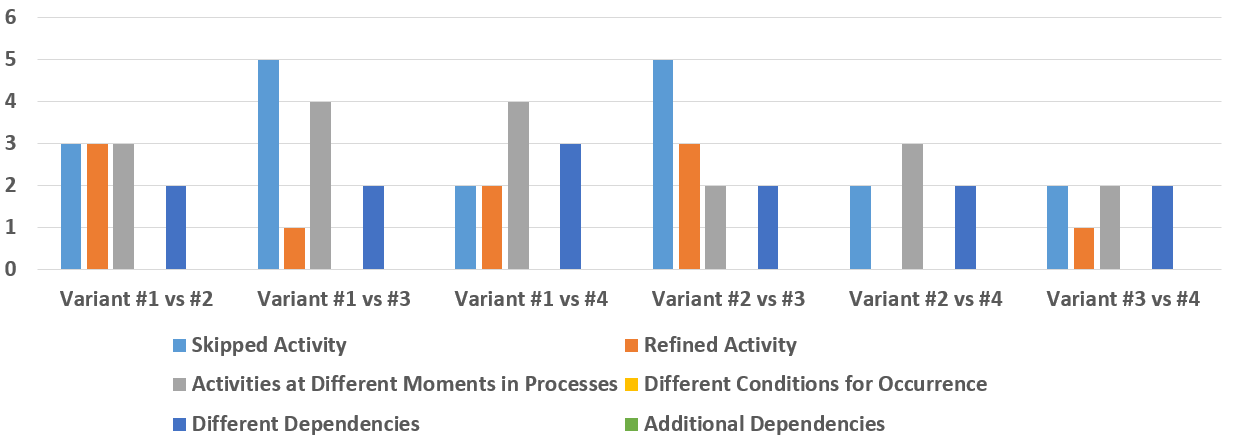
\includegraphics[width=\textwidth]{5_results_discussions/loan-application-process/mismatch-pattern-types}
	\caption{Mismatch pattern types for Loan Application Process variants}
  \label{fig:loan-mismatch-pattern-types}
\end{figure}
 
In \textit{Recommendation Generation} stage, an organization and performance difference threshold is selected as analysis input. For the selected organization's cluster, all other clusters are checked for performing better than the specified threshold. Instead of all mismatch patterns between organizations, only the mismatch patterns that are potential causes of other organizations to perform better are listed. For different threshold values, number of performance indicators that are performing better for the selected organization and spotted mismatch patterns are plotted in Figure~\ref{fig:loan-recommendation-generation-analysis}. 
\begin{figure}
	\centering
	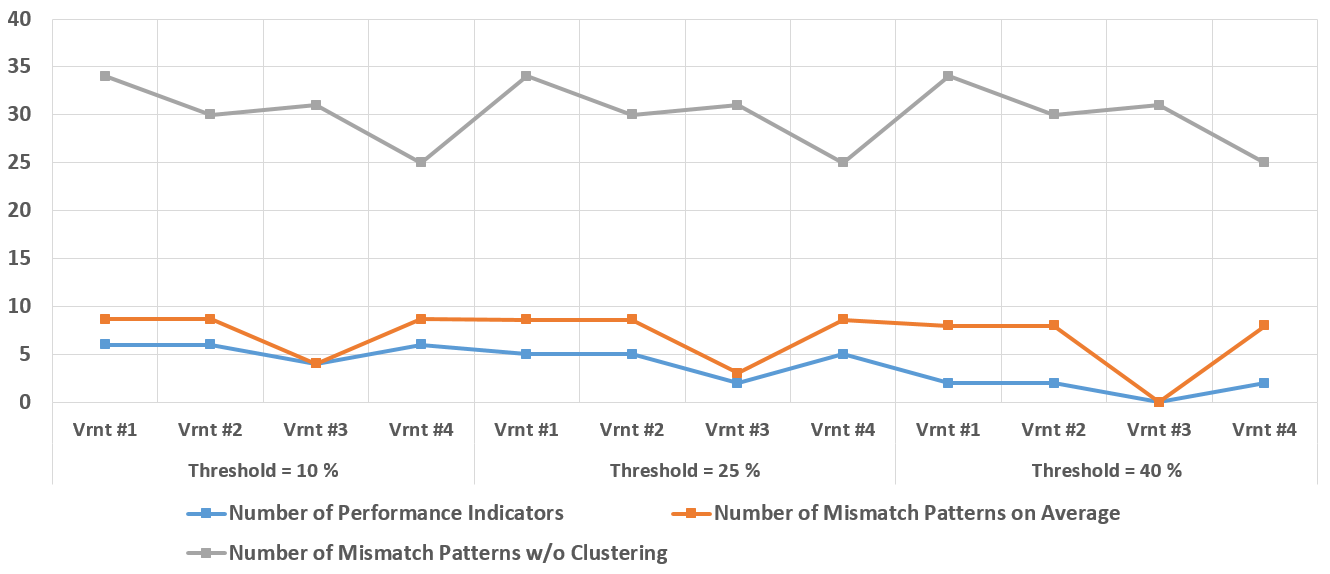
\includegraphics[width=\textwidth]{5_results_discussions/loan-application-process/recommendation-generation-analysis}
	\caption{Recommendation Generation analysis for Loan Application Process dataset}
  \label{fig:loan-recommendation-generation-analysis}
\end{figure}

In order to construct the data in Figure~\ref{fig:loan-recommendation-generation-analysis}, every organization is selected one-by-one with different threshold values. For every analysis, number of performance indicators and average number of mismatch patterns causing them are plotted. In addition, total number of mismatch patterns without clustering for each organization is added to the plot as an upper bound. With the help of this upper bound, responsiveness and degree of helping the user to focus on the performance improvement can be analyzed. As can be seen, for each threshold value, average number of mismatch patterns \textit{with performance indicator clustering} are very low compared to \textit{without clustering}. In other words, when user wants to improve its performance with any threshold, there is significantly less number of mismatch patterns on average to check. This shows the methodology proposed in this thesis can help users to focus on differences between organizations given this dataset. 

\section{Environmental Permit Application Process}
\label{sec:environmental-permit-application-process}
In this section, methodology proposed in this thesis study will be applied on the \textit{Environmental Permit Application Process} dataset \cite{coselog-data} and evaluation results will be presented with a similar approach above. Statistical information about this dataset can be summarized in Table~\ref{table:coselog-process-summary}.

%\caption{Statistical summary of Environmental Permit Application Process dataset}
%\label{table:coselog-process-summary}
 
% As shown in Table~\ref{table:loan-app-process-summary}, total of 475 cases and 2440 events included in this dataset with a fairly even distribution between variants. In the following sections, these variants will be used as organizational logs and the methodology presented in this thesis study will be applied.

\subsection{Methodology Stages}
\label{sec:coselog-methodology}

\subsection{Results}
\label{sec:coselog-results}

\section{Discussions}
\label{sec:discussions}